\documentclass[13pt]{beamer}
\usetheme{Madrid}
\setbeamercovered{invisible}
\setbeamertemplate{navigation symbols}{} 
\usepackage{coordsys} % for number lines
\usepackage{graphicx}
\usepackage{pgfkeys}
\usepackage{caption}
\usepackage{subcaption}
\usepackage{subfloat}
\usepackage{tikz}
\usetikzlibrary{matrix}

% font customization
% \usepackage{mathspec}
% \usepackage{xunicode}
% \usepackage{xltxtra}
% \setmainfont{Gill Sans}
% \setmathsfont(Digits,Latin,Greek){Gill Sans}

%%%%%%%%%%%%%%%%%%%%%%%%%%%%%%%%%%%%%%%%%
\title[Indian Buffet Process]{The Indian Buffet Process}
\author[Bingham and Dickenson]{Eli Bingham\inst{1} \and Matt Dickenson\inst{2}}
\institute[UNC and Duke]{\inst{1} University of North Carolina \and \inst{2} Duke University}
\date{February 10, 2014}


\begin{document}
%%%%%%%%%%%%%%%%%%%%%%%%%%%%%%%%%%%%%%%%%
\begin{frame}
\titlepage
\end{frame}
%%%%%%%%%%%%%%%%%%%%%%%%%%%%%%%%%%%%%%%%%
\begin{frame}
\frametitle{Outline}
\begin{enumerate}
\item Introduction
\item Dirichlet and Chinese Restaurant Processes
\item Beta and Indian Buffet Processes
\item Gibbs sampling
\item Demonstration/Visualization
\item Applications: Choice Behavior and Collaborative Filtering
\item Extensions: Topic Models and Cascading IBP
\item Discussion
\end{enumerate}
\end{frame}
%%%%%%%%%%%%%%%%%%%%%%%%%%%%%%%%%%%%%%%%%
\begin{frame}
\frametitle{Example}

\begin{figure}
\begin{center}
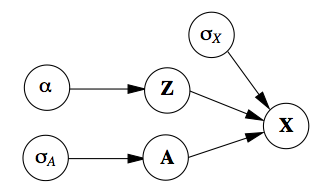
\includegraphics[scale=0.3]{./img/graphical-model-gaussian.png}
\caption{Griffiths and Ghahramani (2011) Figure 7}
\end{center}
\end{figure}

\begin{figure}
\begin{center}
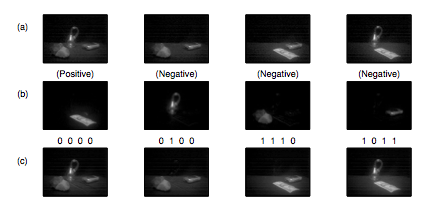
\includegraphics[scale=0.3]{./img/ibp-example-photos.png}
\caption{Griffiths and Ghahramani (2011) Figure 9}
\end{center}
\end{figure}

\end{frame}
%%%%%%%%%%%%%%%%%%%%%%%%%%%%%%%%%%%%%%%%%
\begin{frame}
\frametitle{Motivation}

When and why would we use IBP?

\begin{itemize}
\item As a prior on sparse binary matrices with a countably infinite number of columns
\end{itemize}

\end{frame}
%%%%%%%%%%%%%%%%%%%%%%%%%%%%%%%%%%%%%%%%%
\begin{frame}
\frametitle{Introduction}

Indian Buffet Process:
\begin{enumerate}
\item $N$ customers enter (in sequence) a buffet restaurant with an infinite number of dishes
\item First customer fills her plate with Poisson($\alpha$) number of dishes
\item $i^{th}$ customer samples dishes in proportion to their popularity, with probability $\frac{m_k}{i}$, where $m_k$ is the number of previous customers who sampled dish $k$
\item $i^{th}$ customer then samples a Poisson($\frac{\alpha}{i}$) number of new dishes
\end{enumerate}

\begin{figure}
\begin{center}
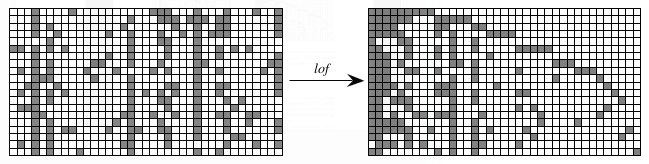
\includegraphics[scale=0.5]{./img/ibp-sorted.png}
\caption{Griffiths and Ghahramani (2011) Figure 5}
\end{center}
\end{figure}

\end{frame}
%%%%%%%%%%%%%%%%%%%%%%%%%%%%%%%%%%%%%%%%%
\begin{frame}
\frametitle{Background: Dirichlet Process}

Finite version (Dirichlet distribution):
\begin{itemize}
\item Assignment of an object to a class is independent of all other assignments: $P(c|\theta) = \prod_{i=1}^N P(c_i|\theta) = \prod_{i=1}^N \theta_{c_i}$
\item $\theta|\alpha \sim \text{Dirichlet}(\frac{\alpha}{K},\ldots,\frac{\alpha}{K})$ (if symettric)
\item $c_i|\theta \sim \text{Discrete}(\theta)$, where Discrete : Bernoulli :: Multinomial : Binomial
\end{itemize}

Integrating out $\theta$: $P(c) = { \prod_{k=1}^K \Gamma(m_k + \frac{\alpha}{K}) \over \Gamma(\frac{\alpha}{K})^K} {\Gamma(\alpha) \over \Gamma(N+\alpha)}$

What happens as $K \rightarrow \infty$?

\begin{figure}
\begin{center}
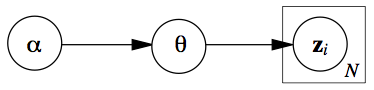
\includegraphics[scale=0.3]{./img/crp-graphical-model.png}
\caption{Griffiths and Ghahramani (2011) Figure 1}
\end{center}
\end{figure}

\end{frame}
%%%%%%%%%%%%%%%%%%%%%%%%%%%%%%%%%%%%%%%%%
\begin{frame}
\frametitle{Background: Chinese Restaurant Process}

\begin{enumerate}
\item $N$ customers enter (in sequence) a restaurant with an infinite number of tables, each with infinite seating
\item First customer sits at first table with probability $\frac{\alpha}{\alpha}=1$
\item $i^{th}$ customer sits at the $k^{th}$ table with probability $\frac{m_k}{i+\alpha-1}$, where $m_k$ is the number of previous customers who sat at table $k$, or a new table with probability $\frac{\alpha}{i+\alpha-1}$
\end{enumerate}

\begin{figure}
\begin{center}
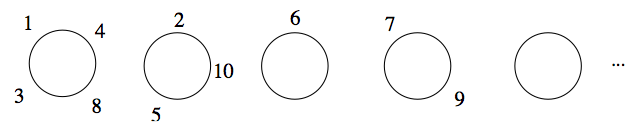
\includegraphics[scale=0.3]{./img/crp-example.png}
\caption{Griffiths and Ghahramani (2011) Figure 2}
\end{center}
\end{figure}

Limitation: each object (customer) can only belong to one class (table).

\end{frame}
%%%%%%%%%%%%%%%%%%%%%%%%%%%%%%%%%%%%%%%%%
\begin{frame}
\frametitle{Beta Process}
% p 1194-5
\end{frame}
%%%%%%%%%%%%%%%%%%%%%%%%%%%%%%%%%%%%%%%%%
\begin{frame}
\frametitle{Indian Buffet Process}
% p 1199
\end{frame}
%%%%%%%%%%%%%%%%%%%%%%%%%%%%%%%%%%%%%%%%%
\begin{frame}
\frametitle{Stick-Breaking Construction of IBP}

\begin{enumerate}
\item Recursively break (an initially unit-length) stick, breaking off a $\text{Beta}(\alpha, 1)$ portion at each step
\item Let each portion of the ``stick'', $\pi_k$ represent the probability of each feature (sorted from largest to smallest)
\end{enumerate}

This helps to show the relation between the Dirichlet process and the IBP. The stick-breaking construction is also useful for defining inference algorithms.

\end{frame}
%%%%%%%%%%%%%%%%%%%%%%%%%%%%%%%%%%%%%%%%%
\begin{frame}
\frametitle{Demo}

\begin{center}
\href{http://mcdickenson.shinyapps.io/ibp-demo}{mcdickenson.shinyapps.io/ibp-demo}
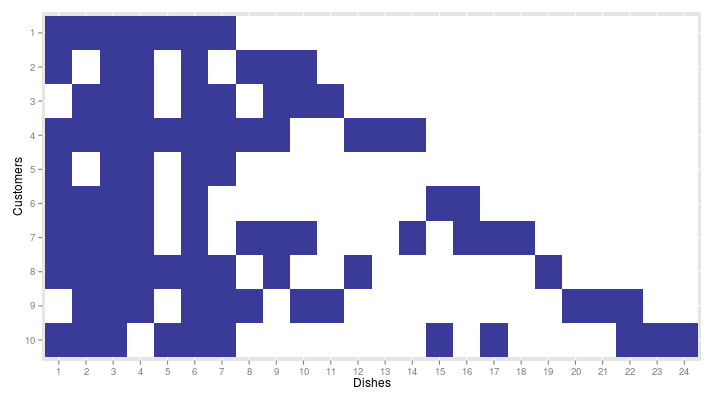
\includegraphics[scale=0.4]{./img/ibp-shiny-demo.png}
\end{center}

\end{frame}
%%%%%%%%%%%%%%%%%%%%%%%%%%%%%%%%%%%%%%%%%
\begin{frame}
\frametitle{Properties of the Resulting Distribution}
% 4.6
\begin{itemize}
\item The ``effective'' dimension $K_+ \sim \text{Poisson}(\alpha H_N)$
\item The number of dishes on each customer's plate is distributed Poisson($\alpha$) (by exchangeability)
\item $\bf{Z}$ remains sparse as $K\rightarrow \infty$: effective dimensions of $\bf{Z}$ are $N \times K_+$, and the expected number of entries is $N\alpha$
\end{itemize}
% note that the third item here is a limitation of the IBP: average number of features $\alpha$ and total number of features $N\alpha$ are directly coupled

\end{frame}
%%%%%%%%%%%%%%%%%%%%%%%%%%%%%%%%%%%%%%%%%
\begin{frame}
\frametitle{Inference by Gibbs Sampling}
% p 1201
\end{frame}
%%%%%%%%%%%%%%%%%%%%%%%%%%%%%%%%%%%%%%%%%
\begin{frame}
\frametitle{Variational Inference}
% sec 6.9
\end{frame}
%%%%%%%%%%%%%%%%%%%%%%%%%%%%%%%%%%%%%%%%%
\begin{frame}
\frametitle{Application 1: Choice Behavior}

% 6.1
\begin{center}
``A Choice Model with Infinitely Many Latent Features'' \\ (G\"{o}r\"{u}r, J\"{a}kel, and Rasmussen, ICML 2006)
\end{center}

\begin{itemize}
\item Customers compare items (e.g. cell phones) based on the (binary) features of each; more features are better
\item Number of features is potentially infinite and ordering is not important, so IBP is used
\item Celebrity example: ``With whom would you prefer to spend an hour of conversation?'' 
\end{itemize}

% \begin{eqnarray*}
% P(f_{ik}=1|f_{-i,k}) &=& {m_{-i,k} + \alpha/K \over N + \alpha/K} \\
% \lim_{K \rightarrow \infty} P(f_{ik}=1|f_{-i,k}) &=& {m_{-i,k} \over N}
% \end{eqnarray*}

\begin{figure}
\begin{center}
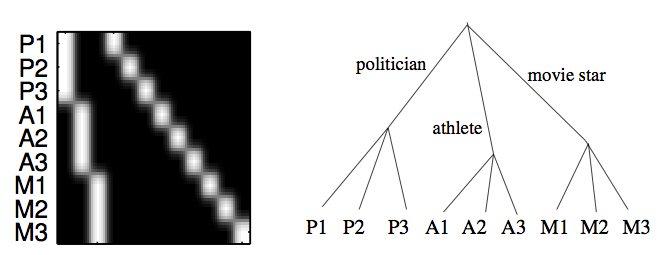
\includegraphics[scale=0.3]{./img/celebrity-example.png}
\caption{G\"{o}r\"{u}r, J\"{a}kel, and Rasmussen (2006) Figure 3}
\end{center}
\end{figure}
% ``We showed empirically that the infinite model (iEBA) can capture the latent structure in the choice data as well as the handcrafted model (tEBA). For data for which we have less prior informa- tion it might not be possible to handcraft a reasonable feature matrix.''

\end{frame}
%%%%%%%%%%%%%%%%%%%%%%%%%%%%%%%%%%%%%%%%%
\begin{frame}
\frametitle{Application 2: Collaborative Filtering}
\end{frame}
%%%%%%%%%%%%%%%%%%%%%%%%%%%%%%%%%%%%%%%%%
\begin{frame}
\frametitle{Extension 1: Topic Modeling}
% Williamson, Wang, Heller, and Blei (2010)

\begin{center}
``The IBP Compound Dirichlet Process \\
and its Application to Focused Topic Modeling'' \\
Williamson, Wang, Heller, and Blei (2010)
\end{center}

Stick-breaking construction:

\begin{eqnarray*}
\mu_k \sim \text{Beta}(\alpha, 1) \\
\pi_k = \prod_{j=1}^k \mu_j \\
b_{m,k} \sim \text{Bernoulli}(\pi_k) 
\end{eqnarray*}


\end{frame}
%%%%%%%%%%%%%%%%%%%%%%%%%%%%%%%%%%%%%%%%%
\begin{frame}
\frametitle{Extension 1: Topic Modeling}
% Williamson, Wang, Heller, and Blei (2010)

\begin{center}
``The IBP Compound Dirichlet Process \\
and its Application to Focused Topic Modeling'' \\
Williamson, Wang, Heller, and Blei (2010)
\end{center}

Focused topic model:
\begin{enumerate}
\item for $k=1,2,\ldots$
  \begin{itemize}
  \item Sample stick length $\pi_k$
  \item Sample relative mass $\phi_k \sim \text{Gamma}(\gamma, 1)$
  \item Draw topic distribution over words: $\beta_k \sim \text{Dirichlet}(\eta)$
  \end{itemize}
\item for $m=1,\ldots,M$
  \begin{itemize}
  \item Sample binary vector $b_m$
  \item Draw total number of words $n^{(m)} \sim NB(\sum_k b_{m,k} \phi_k, 1/2)$
  \item Sample distribution over topics $\theta_m \sim \text{Dirichlet}(b_m \cdot \phi)$
  \item For each word $w_{m,i}, i=1,\ldots,n^{(m)}$
    \begin{enumerate}
    \item Draw topic index $z_{m,i} \sim \text{Discrete}(\theta_m)$ 
    \item Draw word $w_{m,i} \sim \text{Discrete}(\beta_{z_{m_i}})$
    \end{enumerate}
  \end{itemize}
\end{enumerate}

\end{frame}
%%%%%%%%%%%%%%%%%%%%%%%%%%%%%%%%%%%%%%%%%
\begin{frame}
\frametitle{Extension 1: Topic Modeling}
% Williamson, Wang, Heller, and Blei (2010)

\begin{center}
``The IBP Compound Dirichlet Process \\
and its Application to Focused Topic Modeling'' \\
Williamson, Wang, Heller, and Blei (2010)
\end{center}

An advantage of the focused topic model is that it separates the global topic proportions from the distribution over topics within a topic. A rare topic within the corpus can be dominant within a document (e.g. baseball), and a frequent topic can be a small proportion of many documents.

\end{frame}
%%%%%%%%%%%%%%%%%%%%%%%%%%%%%%%%%%%%%%%%%
\begin{frame}
\frametitle{Extension 2: Collaborative Filtering}
% Adams, Wallach, and Ghahramani
\end{frame}
%%%%%%%%%%%%%%%%%%%%%%%%%%%%%%%%%%%%%%%%%
\begin{frame}
\frametitle{Discussion}


Limitations of IBP:
\begin{enumerate}
\item Coupling of average number of features $\alpha$ and total number of features $N\alpha$ (can be overcome with a two-parameter generalization)
\item Computationally complex, can be time-consuming
\end{enumerate}

\begin{figure}
\begin{center}
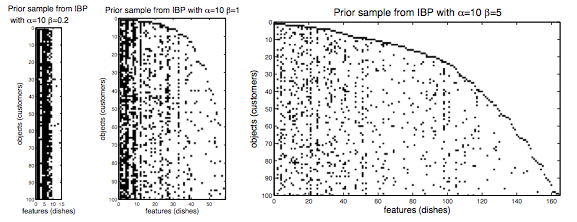
\includegraphics[scale=0.3]{./img/two-parameter-ibp.png}
\caption{Griffiths and Ghahramani (2011) Figure 10}
\end{center}
\end{figure}

\end{frame}
 
% End of slides
\end{document} 
